\section*{Pregunta 3}
\noindent El segundo prototipo debe ser diseñado como una lámina para
proteger un dispositivo electrónico. Dicha lámina debe ser diseñada
en un plano cartesiano limitada por los ejes coordenados del primer
cuadrante y por la gráfica de la función.
\begin{gather*}
  f(x) = 15 - x^2
\end{gather*}
\begin{itemize}
  \item[a.] Determine el centro de masa de dicha lámina. Suba aquí la
    imagen de sus de procesos y desarrollo. No olvide comprobar sus
    respuestas con el Desmos en la siguiente página. Revise la
    grabación de la clase aceca del tema de Centro de gravedad.
  \item[b.] Mediante el uso de plataformas digitales (GEOGEBRA,
    DESMOS, etc), presente gráficamente este prototipo. Use la siguiente página.
\end{itemize}

\subsection*{a. Determine el centro de masa de dicha lámina}
\begin{center}
  \[
    \begin{array}{c@{\hspace{1cm}}|@{\hspace{1cm}}c}
      \begin{aligned}
        & f(x) = 15 - x^2 \\
        & 0 = 15 - x^2 \\
        & x^2 = 15 \\
        & x = \sqrt{15}
      \end{aligned}
      &
      \begin{gathered}
        A = \int_0^{\sqrt{15}} 15 - x^2 dx \\
        A = \left[15x - \frac{x^3}{3}\right]_0^{\sqrt{15}} \\
        A = 10\sqrt{15}
      \end{gathered}
    \end{array}
  \]
  \rule{\textwidth}{0.4pt}
  \begin{align*}
    A \cdot \bar{x} &= \int_0^{\sqrt{15}} x f(x) dx =
    \int_0^{\sqrt{15}} x \left(15 - x^2\right) dx =
    \int_0^{\sqrt{15}} 15x - x^3 dx \\
    A \cdot \bar{x} &= \left[\frac{15x^2}{2} - \frac{x^4}{4}\right] =
    \frac{225}{4} \quad \Bigg| \quad \bar{x} = 1.452
  \end{align*}
  \rule{\textwidth}{0.4pt}
  \begin{align*}
    2A \cdot \bar{y} &= \int_0^{\sqrt{15}} \left(15 - x^2\right)^2 dx
    = \int_0^{\sqrt{15}} 225 + x^4 - 30x^2 dx \\
    2A \cdot \bar{y} &= \left[225x + \frac{x^5}{5} -
    \frac{30x^3}{3}\right]_0^{\sqrt{15}} \approx 464.758 \quad \Bigg|
    \quad \bar{y} \approx 5.999
  \end{align*}
\end{center}

\subsection*{b. Presente gráficamente este prototipo}
\begin{center}
  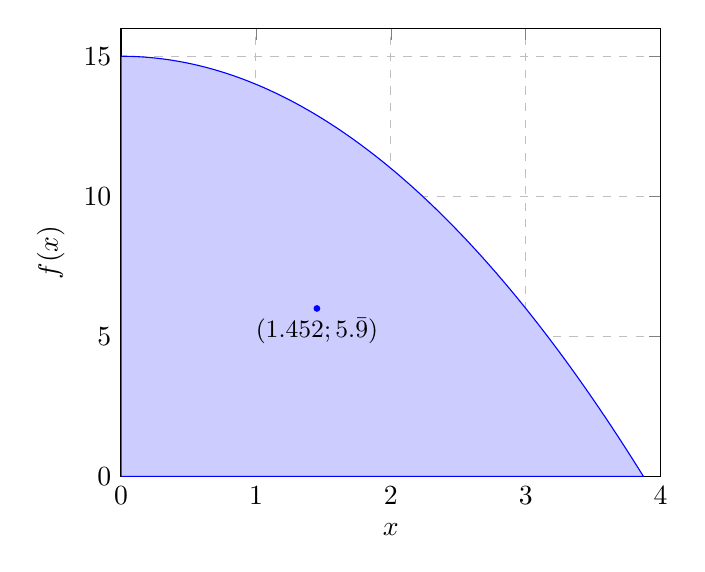
\begin{tikzpicture}
    \begin{axis}[
        xlabel = \(x\),
        ylabel = \(f(x)\),
        xmin = 0, xmax = 4,
        ymin = 0, ymax = 16,
        grid = major,
        grid style = dashed,
      ]

      \addplot[
        domain=0:3.873,
        samples=100,
        color=blue,
        fill=blue!20,
      ]
      {15 - x^2} \closedcycle;

      \addplot[
        only marks,
        mark=*,
        mark size=1pt,
        color=blue,
      ] coordinates {(1.452, 5.999)};
      \node[below] at (axis cs:1.452,5.999) {\small $(1.452; 5.\bar{9})$};
    \end{axis}
  \end{tikzpicture}
\end{center}
